\documentclass[./../../paper.tex]{subfiles}
\graphicspath{{\subfix{./../../figures/}}}

\begin{document}



% \begin{figure}[htb]
%     \centering
%     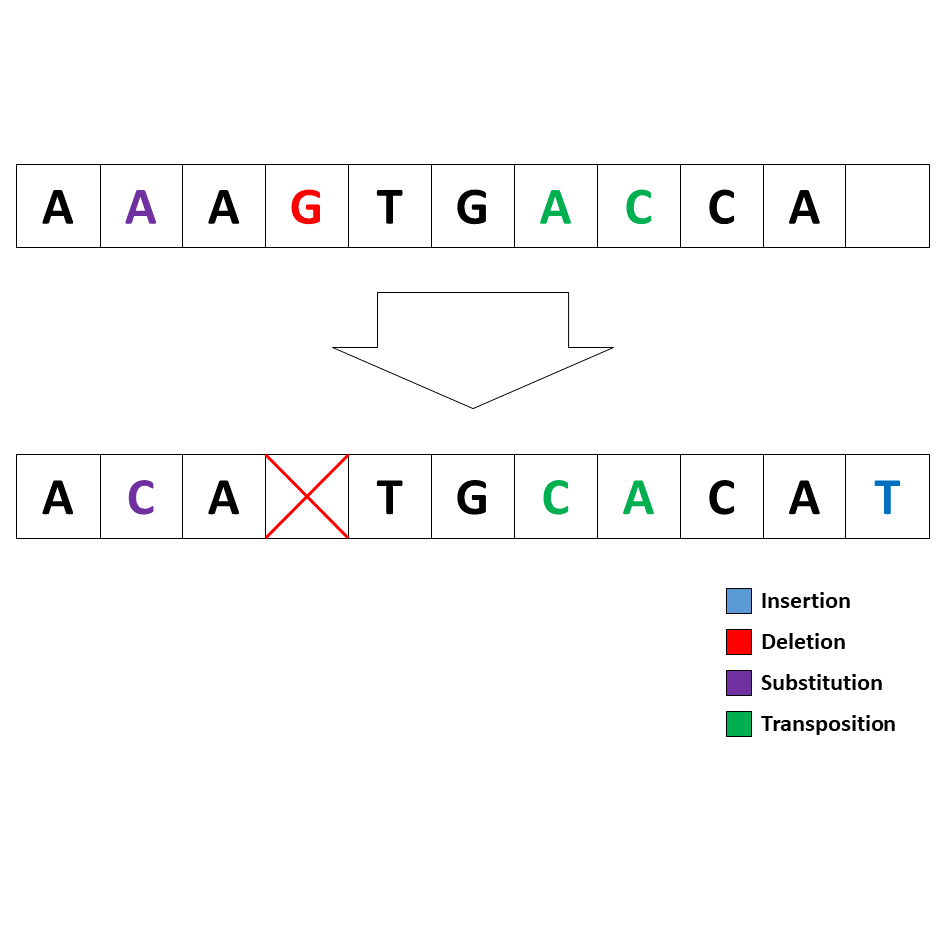
\includegraphics[width=0.99\textwidth]{figures/Graphics/Slide6.PNG}
%     \caption{This figure exemplifies the differeneces between the normal DL-distance and this one used.}
%     \label{fig:image_with_dl}
% \end{figure}

% \needsfigure{fig:image_with_dl}{This figure exemplifies the differeneces between the normal DL-distance and this one used.}

\noindent In order to reflect these differences in attribute values, we introduce a modified version of the \gls{damerau_levenshtein}, that not only reflects the difference between two process instances, but also the attribute values. We achieve this by introducing a cost function $\editCost$, which applies to a normed vector-space\footnotemark. Concretely, we formulate the modified \gls{damerau_levenshtein} as shown in \autoref{eq:modified_dl}. For the remainder, we refer to this edit-distance as \gls{SSDLD}.\footnotetext{A normed vector-space is a vector space, in which all vectors have the same dimensionality. For instance, if all vectors have three dimensions, we can call the vector-space \emph{normed}.}
% TODO: Introduce a with a dash above to compare activities instead of the vector
% Make zero thicker to indicate a null vector
\begin{align}
    \label{eq:modified_dl}
    d_{a, b}(i, j) & =\min
    \begin{cases}
        \editDistance{i-1}{j  }+\editCostFunctionNoA & \text { if } i>0                                            \\
        \editDistance{i  }{j-1}+\editCostFunctionNoB & \text { if } j>0                                            \\
        \editDistance{i-1}{j-1}+\editCostFunctionBoth & \text { if } i, j>0   \\ & \text { \& } \overline{a}_i=\overline{b}_j                                       \\
        \editDistance{i-1}{j-1}+ \editCostFunctionNoB +\editCostFunctionNoA  & \text { if } i, j>0  \\ & \text { \& } \overline{a}_i \neq \overline{b}_j                                       \\
        \editDistance{i-2}{j-2}+\editCostFunction{a_i}{b_{j-1}} + \editCostFunction{a_{i-1}}{b_j} & \text { if } i, j>1 \\ 
        & \text { \& } \overline{a}_i=\overline{b}_{j-1} \\ 
        & \text { \& } \overline{a}_{i-1}=\overline{b}_j \\
        0                                 & \text { \& } i=j=0                                          
    \end{cases} 
\end{align}

\noindent Here, $d_{a, b}(i, j)$ is the recursive form of the Damerau-Levenshtein-Distance. $a$ and $b$ are sequences and $i$ and $j$ specific elements of the sequence. $cost(a,b)$ is a cost function which takes the attribute values of $a$ and $b$ into account. 
The first two terms correspond to a deletion and an insertion from $a$ to $b$. The idea is to compute the maximal cost for that the wrongfully deleted or inserted event. 
The third term adds the difference between two events with identical activities $\overline{a}_i$ and $\overline{b}_j$. As mentioned earlier, two events that refer to the same activity can still be different due to event attributes. The distance between the event attributes determines \emph{how} different these events are. 
The fourth term handles the substitution of two events. Here, we compute the substitution cost as the sum of an insertion and a deletion. 
The fifth term computes the cost after transposing both events. This cost is similar to term 3 only that we now consider the differences between both events after they were aligned. The last term relates to the stopping criterion of the recursive formulation of the \gls{damerau_levenshtein}.  


\end{document}